\documentclass[letterpaper,12pt]{article}
\usepackage[T1]{fontenc}
\usepackage{mathptmx}

% unit definition
\usepackage{siunitx}
% \sisetup{load-configurations = abbreviations}
\DeclareSIUnit\inch{in}
\DeclareSIUnit\ft{ft}
\DeclareSIUnit\Rank{^{\circ} R}
\DeclareSIUnit\Faren{^{\circ} F}
\DeclareSIUnit\lbm{lb_{m}}
\DeclareSIUnit\lbf{lb_{f}}
\DeclareSIUnit\torr{Torr}
\DeclareSIUnit\gallon{gal}
\DeclareSIUnit\slug{slug}
\DeclareSIUnit\knots{kts}
\DeclareSIUnit\miles{mi}


% hyperlink formatting
\usepackage{hyperref}
\hypersetup{
    colorlinks=true,
    linkcolor=red,
    urlcolor=purple,
    citecolor=blue
}


% Other general packages
\usepackage{setspace}
\usepackage{graphicx}
\usepackage{float}
\usepackage{amsmath}
\usepackage{amssymb}
\usepackage{tabto}
\usepackage{booktabs, tabularx}
\usepackage{enumitem}
\usepackage{gensymb}
\usepackage{cancel}
\usepackage{tikz}
\usepackage{pgfplots}
\usepackage{appendix}
\usepackage[labelfont=bf, font={normalsize,stretch=1}]{caption}
\usepackage[letterpaper, margin=1.0in]{geometry}
\usepackage[utf8]{}
\usepackage{indentfirst}
\setlength{\parindent}{0.25in}

%Heading format
\usepackage{titlesec}
\titleformat*{\section}{\normalsize\bfseries}
\titleformat*{\subsection}{\normalsize\bfseries}
\titleformat*{\subsubsection}{\normalsize\bfseries}

%Page Numbers
\usepackage{fancyhdr} 
\pagestyle{fancy}
\fancyhf{}
\fancyheadoffset{0cm}
\renewcommand{\headrulewidth}{0pt} 
\renewcommand{\footrulewidth}{0pt}
\fancyhead[R]{\thepage}
\pagenumbering{arabic}

%listings package for code
\usepackage{listings}
\usepackage{xcolor}

% bibliography formatting
\usepackage{etoolbox}
\patchcmd{\thebibliography}{\section*{\refname}}{}{}{}
\setstretch{2}

% color definitions
\definecolor{dblue}{HTML}{145680}
\definecolor{dred}{HTML}{801414}
\definecolor{dgreen}{HTML}{148014}
\definecolor{bgcode}{rgb}{0.95,0.95,0.95}
\definecolor{codegreen}{rgb}{0,0.6,0}
\definecolor{codegray}{rgb}{0.5,0.5,0.5}
\definecolor{codepurple}{rgb}{0.58,0,0.82}
\definecolor{backcolour}{rgb}{0.95,0.95,0.92}

\lstdefinestyle{mystyle}{
    backgroundcolor=\color{backcolour},
    commentstyle=\color{codegreen},
    keywordstyle=\color{magenta},
    numberstyle=\tiny\color{codegray},
    stringstyle=\color{codepurple},
    basicstyle=\ttfamily\footnotesize,
    breakatwhitespace=false,
    breaklines=true,
    captionpos=b,
    keepspaces=true,
    numbers=left,
    numbersep=5pt,
    showspaces=false,
    showstringspaces=false,
    showtabs=false,
    tabsize=2
}
\lstset{style=mystyle}

\pgfplotsset{compat=1.17}

% NOTES
%  - Double spacing (always fix for figures and tables though)
%  - for tables, remember to make them single spaced using \renewcommand{\arraystretch}{1}
%  - Always pull from GitHub to Overleaf when there are commits to be pulled (Menu > GitHub > PULL)
%  - for REFERENCES, use \cite{<label>} to link the reference.

% % TABLE TEMPLATE
% \begin{table}[H]
%     \begin{center}
%     \setstretch{1} 
%     \caption{\textbf{<caption here>}} \label{table:<label here>}
%     \begin{tabular}{|p{0.3in}|p{1in}|p{1in}|} % set column nums and width
%         \hline \textbf{No.} & \textbf{Item} & \textbf{Weight} \\ \hline % column headers
%         1 & Hot dogs & 2 lbs \\ \hline
%     \end{tabular}
%     \end{center}
% \end{table}

\begin{document}

%%% Title Pa
\begin{center}
    {\Large\textbf{AE 484 Homework 2}}\\
    Anshuk Chigullapalli, George Petrov, Kenneth Tochihara, Jeffery Zhou\\

\end{center}


\section{Group name and leader}
% Determine a group name and vote/select a group leader

    \textbf{Group Name:} Illinois Air Society % subject to change
    \textbf{Group Leader:} George Petrov % subject to change

\section{Existing tailless RC aircraft}
% Search the internet or publications and evaluate 4 flying wing (tailless) R/C or UAV aircraft. In a table determine the following: Name of the aircraft, Wing planform area, Winglet planform area, weight of the aircraft, wing loading (W/S), Wing sweep, Wing taper ratio, wing root chord length, wing tip chord length, wing span, motor position (tractor or pusher), motor size (power), link or reference where information was gathered. Note that many of these quantities are estimates and may need to be scaled from pictures or schematics.

    \begin{table}[H]
        \begin{tabular}{|c|c|c|c|c|} % set column nums and width
            \hline \textbf{Name} & \textbf{Wing planform area} & \textbf{Winglet planform area} & \textbf{Weight} & \textbf{Loading (W/S)} \\ \hline % column headers
             & & & & \\ \hline
             & & & & \\ \hline
             & & & & \\ \hline
             & & & & \\ \hline
        \end{tabular}
    \end{table}
    
    \begin{table}[H]
        \begin{tabular}{|c|c|c|c|c|c| } % set column nums and width
            \hline \textbf{Name} & \textbf{Sweep} & \textbf{Taper ratio} & \textbf{Root chord length} & \textbf{Tip chord length} & \textbf{Span} \\ \hline % column headers
             & & & & & \\ \hline
             & & & & & \\ \hline
             & & & & & \\ \hline
             & & & & & \\ \hline
        \end{tabular}
    \end{table}
    
    \begin{table}[H]
        \begin{tabular}{|c|c|c|c| } % set column nums and width
            \hline \textbf{Name} & \textbf{Motor position} & \textbf{Motor size} & \textbf{Reference} \\ \hline % column headers
             & & & \\ \hline
             & & & \\ \hline
             & & & \\ \hline
             & & & \\ \hline
        \end{tabular}
    \end{table}

\section{Objectives and constraints}
% Write a paragraph summarizing objectives and what constraints are place on your design. In addition to the mission objectives create bulleted items of design objectives and constraints which your vehicle should meet with numerical values when possible. Mark each numbered bulleted item with a 1 thru 3 number indicating the level of importance (1-vehicle must meet item, 2-some flexibility in item, 3-optional).

    The overall objective of the mission is to design and build a mini-UAV that deploys a vial of vaccine to a remote area. This UAV shall be hand-launched and shall land without any landing gears. Testing shall remain within line-of-sight (LOS) and shall abide by the Academy of Model Aeronautics (AMA) guidelines. The UAV shall be tailless with only two control surfaces. Propeller/Motor/Speed Controller/Battery combinations are provided and shall be utilized within the design. This UAV shall be capable of achieving altitude quickly. The UAV's wings shall be made with Balsa reinforced foam with a fiberglass covering and shall be propelled with a tractor or pusher configuration.
    
    \begin{itemize}
        \item \textbf{Max Altitude (1):} 400 ft
        \item \textbf{Flight Time (2):} 15 min
        \item \textbf{Top Speed (2):} 40 mph
        \item \textbf{Max Thickness (3):} 1.75 in
        \item \textbf{Max Wingspan (1):} 70 in
        \item \textbf{Max Weight (3):} 3 lbs
    \end{itemize}


\section{Individual vehicle concepts}
% Each individual in your group must present one vehicle concept. Each individual should present a three-view drawing (CAD preferred, but very nice ruler and template drawn sketches acceptable) and isometric view of their vehicle configuration the individual proposes with basic (overall) dimensions to ascertain the general size and shape. Indicate which individual is responsible for each design (points may be deducted from the overall grade for individuals who do not have a professional presentation of their concept).

    The drawings of each individual member's CAD designs are attached at the end of the assignment.

\section{Weight and wing loading of vehicle concepts}
% Estimate the weight and wing loading of each concept aircraft (take-off weight). Be sure to include all instrumentation, cargo, battery, etc. in your analysis. Also indicate how you estimated the weight of the structure (i.e. fuselage, spars, skin, bulkheads, winglets, etc.) in the concept drawings. Be sure to include a table with all the weights of the components clearly presented and example calculations of estimated values
    
    \subsection{Anshuk}
    \subsection{George}
    \subsection{Kenneth}
    \subsection{Jeffery}
        % \includepdf[pages=-,scale=0.75,angle=90]{../jeffery/ktt3_aircraft.pdf}

\section{Vehicle concept evaluation}
% The group should evaluate each vehicle design writing down, as bulleted items, how well each design meets the bulleted items in question one. Also write down (bullet points) three major Pros and three major Cons for each design.

    \subsection{Anshuk}
    \subsection{George}
    \subsection{Kenneth}
        
        \begin{itemize}
            \item Meeting objectives
            \begin{itemize}
                \item 
            \end{itemize}
            \item Pros
            \begin{itemize}
                \item 
            \end{itemize}
            \item Cons
            \begin{itemize}
                \item 
            \end{itemize}
        \end{itemize}
        
    \subsection{Jeffery}

\section{Proposed designs}
% Get together virtually as a group and propose the top 2 designs for the mission described in the problem statement. Describe why these were selected as the best designs by the group. Be prepared to discuss all of the designs and the preferred designs in the group meeting on Monday (02/07/2022).

    \subsection{Design 1}
    \subsection{Design 2}

\section{Group member contributions}
% Make a table indicating how each group member contributed to the report

    \begin{table}[H]
        \begin{center}
        \begin{tabular}{ | p{2in} | p{4in}| } 
            \hline
            \textbf{Group Member} & \textbf{Contribution} \\  \hline
            Anshuk Chigullapalli & \\ \hline
            George Petrov & \\ \hline
            Kenneth Tochihara & \\ \hline
            Jeffery Zhou & \\ \hline
        \end{tabular}
        \end{center}
    \end{table}

% \includepdf[pages=-,angle=90]{../anshuk/ktt3_aircraft.pdf}
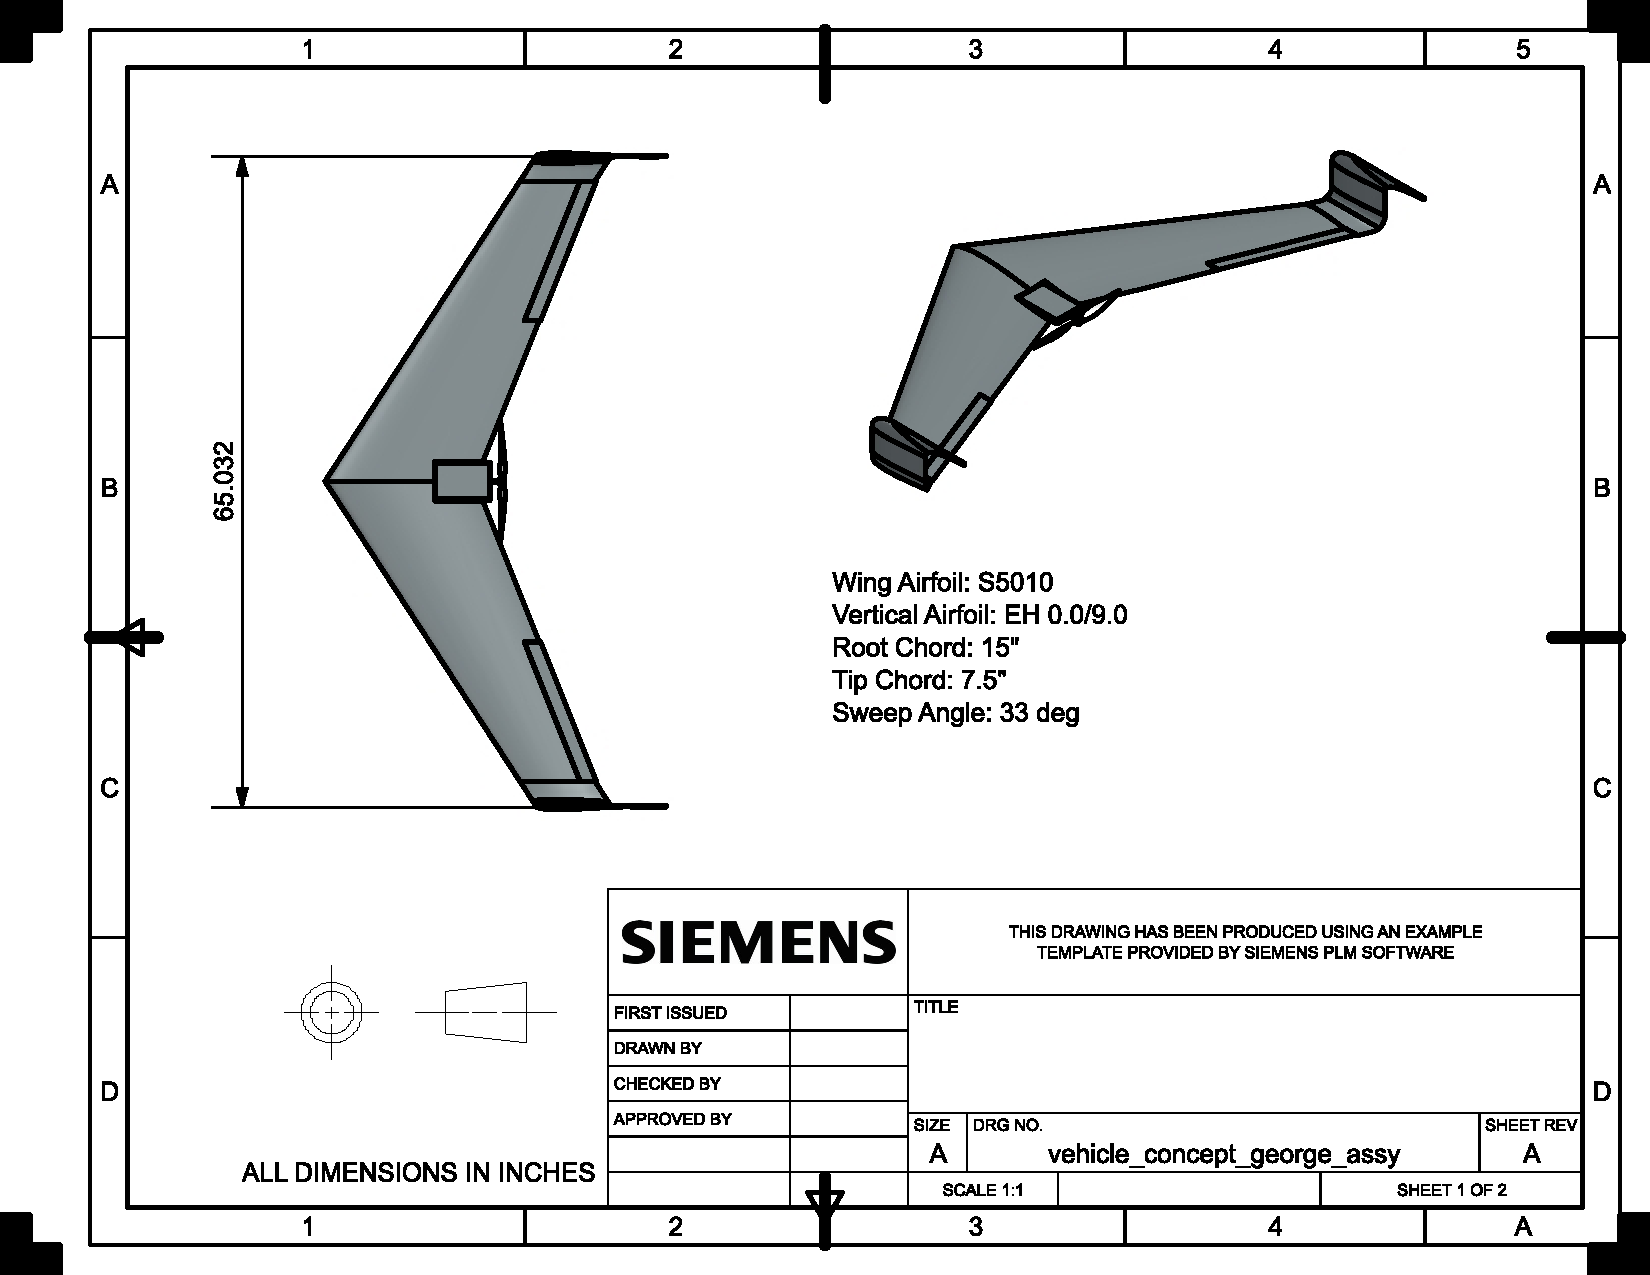
\includepdf[pages=-,angle=90]{../george/Drawings/gpetrov2_vehicle_concept_george_assy.pdf}
\includepdf[pages=-,angle=90]{../kenneth/ktt3_aircraft.pdf}
% \includepdf[pages=-,angle=90]{../jeffery/ktt3_aircraft.pdf}
    
\end{document}